\chapterimage{orange2.jpg}
\chapterspaceabove{6.75cm} 
\chapterspacebelow{7.25cm} 
\chapter{Relations, Abstract Algebra, and Category Theory Introduction}


In this chapter, we will look into common search and sorting algorithms in computer science. This could
be treated as an extension to prior knowledge in this book, as almost every chapter are involved in the
analysis and proof of these algorithms. Stay calm if you find it a little difficult, since it takes some
time for everyone to fully understand the notions. Some of you may think it's quite hilarious to put 
sorting and searching algorithm in a chapter about discrete math, but they are exactly the algorithms that
requires to be analyzed using the most mathematical tools. While the foundation of which is not just what
have been covered in previous chapters, but also.

\section{Relations}
    \subsection{Equivalent Relation}

    \subsection{Inverse Relation}

    \subsection{Recursive Relation}

    \subsection{$n$-ray Relation}

    \subsection{Closure}




\section{Searching algorithms}
    The very first thing we need to do is figure out what is searching, before we do any math.
    \begin{definition}[Searching algorithm]
        Given an array \( A[1], A[2], A[3], \ldots, A[n] \) and a target value \( T \), find an index \( j \) where \( T = A[j] \) or determine that no such index exists because \( T \) is not in the array \( A \).
    \end{definition}
    \subsection{Searching in Unordered Array List}
    We proceed to analyze the most common case, where we need to find the element $T$ from an unordered 
    array. In this case, what we need to do is just like counting numbers. We will check each element in
    the array $A$, from $A[1]$ to $A[n]$, until we find $T$. This way of reaching in pure sequential 
    order is called \textbf{Linear Search}. The pseudocode is shown below.
    \begin{algorithm}
        \caption{Linear search for a target value in an array}
        \begin{algorithmic}[1]
        \Procedure{LinearSearch}{$A, T$}
            \For{$j = 1$ to $j=n$}
                \If{$A[j] == T$}
                    \State \Return $j$
                \EndIf
            \EndFor
            \State \Return $\text{``not found''}$
        \EndProcedure
        \end{algorithmic}
        \end{algorithm} 
    This is the easiest  algorithm in this book, and it is clear that for an array of size $n$, this 
    algorithm has a time complexity of $O(n)$ in the worst cases. Now consider that, what if we are lucky
    enough to find our target $T$ in the very first element in the array? Actually, computer scientists
    have the other notation to show the best-case performance of a algorithm, which is $\omega$ notation.
    \begin{notation}[Omega Notation]
        The Omega notation describes the lower bound of an algorithm's running time. 
        It measures the best-case scenario, at least this fast. For a given function g(n), 
        we denote $\omega(g(n))$ the set of functions:
        \[
        \Omega(g(n)) = \{ f(n) : \exists c > 0, n_0 > 0 \text{ such that } 0 \leq cg(n) \leq f(n) \text{ for all } n \geq n_0 \}
        \]
    \end{notation}
    Yet there is another notation to show the overall, or average performance of an algorithm.
    \begin{notation}[Theta Notation]
        The Theta notation tightly bounds a function from above and below, meaning it defines an algorithm's running time both in the best and worst cases. For a given function $g(n)$, we denote $\Theta(g(n))$ the set of functions:
        \[
        \Theta(g(n)) = \{ f(n) : \exists c_1 > 0, c_2 > 0, n_0 > 0 \text{ such that } 0 \leq c_1g(n) \leq f(n) \leq c_2g(n) \text{ for all } n \geq n_0 \}
        \]
    \end{notation}
    Theta notation is used to evaluate the average time complexity of executing an algorithm. For instance,
    we use $\bar{p}$ to denote the average of accessed elements. We have:
    $$\bar{p} = \frac{1}{n} \sum_{i=i}^{n}i = \frac{1}{n}\times\frac{n(n+1)}{2}=\frac{n+1}{2}$$
    Which means this algorithm has $\Theta(\frac{n+1}{2})$ time complexity.
    \subsection{Searching in Ordered Array List}
    It seems that we do not have any better way to design a more efficient algorithm for finding target in 
    unordered array. Now we will discuss the case for an ordered array.
    \begin{definition}
        An ordered array refers to an array $A$ that satisfies $A[1]\leq \cdots \leq A[n]$ or $A[1]\geq 
        \cdots, \geq A[n]$.
    \end{definition}
    In this case, the target $T$ and any random element $A[n]$ in the array has the following properties
    \begin{itemize}
        \item  If \( T < A[i] \), then \( T \) cannot occur among \( A[i], A[i + 1], \ldots, A[n] \), and we need only search the list from \( A[1] \) to \( A[i - 1] \)
        \item  If \( A[i] < T \), then \( T \) cannot occur among \( A[1], A[2], \ldots, A[i] \), and we need only search the list from \( A[i + 1] \) to \( A[n] \)
    \end{itemize}
    If we adopt a policy of making the worst case as favorable as we can, we should
    probe in the middle (or as near to the middle as possible) of the list (or sublist) we're
    searching. Then, if we don't find the target there, we will have at most half the list to
    search.
    
    Suppose the partition of the original list we are searching in is from $A[p]$ to $A[q]$. We can get
    the median by $\frac{p+q}{2}$, however, when $p+q$ is odd, we cannot get a valid integer as position
    of element. As a result, we probe $A[i]$ where $i = \lfloor \frac{p+q}{2} \rfloor$ instead. 
    The resulting search algorithm where we probe in the middle of the current
    sublist is \textbf{Binary Search}.
    \begin{algorithm}[H]
        \caption{Binary Search for a target value in a sorted array}
        \begin{algorithmic}[1]
        \Procedure{BinarySearch}{$A, T$}
            \State $p \gets 1$
            \State $q \gets n$
            \While{$p \leq q$}
                \State $j \gets \left\lfloor (p + q) / 2 \right\rfloor$
                \If{$A[j] == T$}
                    \State \Return $j$
                \ElsIf{$A[j] < T$}
                    \State $p \gets j + 1$
                \Else
                    \State $q \gets j - 1$
                \EndIf
            \EndWhile
            \State \Return $\text{``not found''}$
        \EndProcedure
        \end{algorithmic}
        \end{algorithm}
    \begin{remark}
        If this code is a little confusing for you, you may check \href{https://www.cs.usfca.edu/~galles/visualization/Search.html}{here}
        for complete visualization of binary search.
    \end{remark}
    
    Walkthrough with $n = 12$ and $A = (3, 5, 8, 8, 9, 16, 29, 41, 50, 63, 64, 67)$. 

    If $T=99$, then, we can show the variables involved in a table.
    \begin{table}[h!] 
        \label{bisearch1}
        \centering
        \begin{tabular}{cccccc}
        \toprule
        \( p \) & \( j \) & \( q \) & \( A[j] \) & relation     & output         \\
        \midrule
        1       & 6       & 12      & 16         & \( A[j] < T \) & -             \\
        7       & 9       & 12      & 50         & \( A[j] < T \) & -             \\
        10      & 11      & 12      & 64         & \( A[j] < T \) & -             \\
        12      & 12      & 12      & 67         & \( A[j] < T \) & -             \\
        13      & -       & 12      & -          & -              & \( T \) is not in \( A \) \\
        \bottomrule
        \end{tabular}
        \caption{Binary Search Iterations}
        \end{table}
        Suppose the sublist we're searching is from \( A[p] \) up to \( A[q] \) of length \( k = q - p + 1\) and we probe unsuccessfully at \( A[j] \):
        $$\underbrace{A[p]\ldots A[j-1]}_{k1}\quad\text{A}[j]\quad\underbrace{A[j+1]\ldots A[q]}_{k2}$$
        
        If \( A[j] \geq T \), then we will search from \( A[p] \) up to \( A[j-1] \) of length \( k_1 = j - p \). \\
        
        If \( A[j] < T \), then we will search from \( A[j+1] \) up to \( A[q] \) of length \( k_2 = q - j \). \\
        
        We would like \( k_1 \) and \( k_2 \) to be equal, but if that's not possible (because \( q - p \) is odd), let's consistently make \( k_1 \) the smaller value.
        $\text{How should we choose }  j  \text{ so that }  k_1 \leq k_2  \text{ and }  k_2$  is as small as possible?
        To make \( k_2 = q - j \) as small as possible, we need to make \( j \) as large as possible. We want
        
        \[ k_1 + k_2 \leq k_2 + k_2, \]
        that is,
        \[ q - p \leq 2(q - j) = 2q - 2j \]
        or
        \[ 2j \leq 2q - (q - p) = q + p. \]
        
        The largest integer \( j \) such that \( j \leq (q + p)/2 \) is \( \lfloor (q + p)/2 \rfloor \), and this is the \( j \)-value used in the algorithm.
        \begin{theorem}[Binary Search Sublist Lengths] \label{sublistlen}
            On each iteration of Binary Search with \( j = \left\lfloor \frac{p + q}{2} \right\rfloor \), the lengths of the sublists will be \( k_1 = \left\lfloor \frac{k - 1}{2} \right\rfloor \) such that \( k_1 \leq k_2 = \left\lceil \frac{k - 1}{2} \right\rceil \leq \frac{k}{2} \).
            \end{theorem}
            
            \begin{proof}
            Since \( j \leq \frac{q + p}{2} < j + 1 \), subtracting \( p \) from each of these three expressions gives
            \begin{align*}
            j - p &\leq \frac{q + p}{2} - p < j - p + 1 \\
            k_1 &\leq \frac{q - p}{2} < k_1 + 1.
            \end{align*}
            Thus, \( k_1 = \left\lfloor \frac{q - p}{2} \right\rfloor = \left\lfloor \frac{k - 1}{2} \right\rfloor \).
            
            Because \( k_1 + k_2 = k - 1 \), we know that
            \begin{itemize}
            \item if \( k \) is odd, say \( k = 2r + 1 \), then \( k - 1 = 2r \) and \( k_1 = r = k_2 < \frac{k}{2} \),
            \item if \( k \) is even, say \( k = 2r \), then \( k - 1 = 2r - 1 \) and \( k_1 = r - 1 < r = k_2 = \frac{k}{2} \).
            \end{itemize}
            Thus, \( k_1 = \left\lfloor \frac{k - 1}{2} \right\rfloor \leq k_2 = \left\lceil \frac{k - 1}{2} \right\rceil \leq \frac{k}{2} \).
            \end{proof}

            \begin{theorem}[Binary Search Termination]
                Binary Search terminates after at most \(\lceil \lg(n) \rceil + 1\) probes.
                \end{theorem}
                
                \begin{proof}
                Let \( w = \lfloor \lg(n) \rfloor \). If, in some instance, Binary Search has not terminated after \( w \) (unsuccessful) probes, then the current value of \( p \) must be \( \leq \) the current value of \( q \), and the length of the current sublist, \( k \), must be \( \leq n/2^w \).
                \[ // \text{Prove this by MI.} \]
                Since \( w \leq \lg(n) < w + 1 \),
                \[ 2^w \leq n < 2 \times 2^w \]
                \[ // \text{then dividing each by } 2^w \]
                \[ 1 \leq n/2^w < 2. \]
                \[ // \text{which implies that } k = 1 \]
                
                For the next iteration, \( p = q \) and so \( j = p \).
                \[ // \text{And we probe the one remaining entry in } A. \]
                
                If \( A[j] < T \), then \( p \leftarrow j + 1 > q \), so Binary Search terminates after this probe; if \( A[j] > T \), then \( q \leftarrow j - 1 < p \), so Binary Search terminates after this probe; and if \( A[j] = T \), then Binary Search terminates after this one last probe.
                
                Therefore, Binary Search terminates after at most \(\lceil \lg(n) \rceil + 1\) probes.
                \end{proof}
    To show that the binary search algorithm is correct, we also need to show its \textbf{loop invariant}.
        \begin{definition}
            In computer science, a loop invariant is a logical assertion that is true before and after 
            each iteration of a program loop. It is a condition that is true at the beginning and 
            end of every iteration of a loop.
        \end{definition}
    Assume that $T$ is in $A$ and $T=A[i]$, $i \in [p, q]$.
    \begin{theorem}[Loop Invariance of Binary Search]
        After $k$ iterations of the loop, if $T$ = $A[i]$, then $p\leq i \leq q$.
    \end{theorem}
    \begin{proof}
        By Mathematical Induction on \(k\) where \(k \in \{0..\}\)

\textbf{Step 1.} After \(k = 0\) iterations of the loop, that is, before the loop is done once
\[ p = 1 \quad \text{and} \quad q = n, \]
and therefore,
\[ \text{if} \quad T = A[i] \quad \text{then} \quad p \leq i \leq q. \quad (\text{P}(0) \text{ is True}) \]

\textbf{Step 2.} Assume \(\exists w \in \mathbb{N}\) such that
after \(w\) iterations of the loop, if \( T = A[i] \), then \( p \leq i \leq q \). \quad (\text{This is P}(w).)

\textbf{Step 3.} Suppose there is another iteration, the \( w + 1^{st} \).
That is, \( T \) has not been found in \( w \) unsuccessful probes, and now, \( p \leq q \).
On the next iteration, we calculate a new \( j \)-value,
\[ j_{\text{new}} \leftarrow \left\lfloor \frac{(p + q)}{2} \right\rfloor \]

Since \( p \leq q \),
\[ p + p \leq p + q \leq q + q \]
and
$$p\ =\ \frac{p+p}{2} \leq \frac{p+q}{2} \leq \frac{q+q}{2} =q$$
and so \( p \leq j_{\text{new}} \leq q \).
In fact, if \( p = q \), then \( j_{\text{new}} = p \), and if \( p < q \), then \( p \leq j_{\text{new}} < q \).

In the remainder of the proof, we will let \( p^* \) and \( q^* \) denote the values of \( p \) and \( q \) at the end of the iteration. There are three cases to consider:

\textbf{Case 1.} If \( A[j_{\text{new}}] < T \), then \( T \) cannot occur at or before position \( j_{\text{new}} \) hence
\[ \text{if} \quad T = A[i] \quad \text{then} \quad p < j_{\text{new}} + 1 \leq i \leq q. \quad \text{Here} \quad p^* = j_{\text{new}} + 1 \quad \text{and} \quad q^* = q. \]

\textbf{Case 2.} If \( A[j_{\text{new}}] > T \), then \( T \) cannot occur at or after position \( j_{\text{new}} \) hence
\[ \text{if} \quad T = A[i] \quad \text{then} \quad p \leq i < j_{\text{new}} - 1 < q. \quad \text{Here} \quad p^* = p \quad \text{and} \quad q^* = j_{\text{new}} - 1. \]

\textbf{Case 3.} If \( A[j_{\text{new}}] = T \), then neither \( p \) nor \( q \) are changed hence, from Step 2
\[ \text{if} \quad T = A[i] \quad \text{then} \quad p \leq i \leq q. \quad \text{In this case,} \quad p^* = p \quad \text{and} \quad q^* = q. \]

Therefore, after this next iteration,
\[ \text{if} \quad T = A[i] \quad \text{then} \quad p^* \leq i \leq q^*. \quad \text{in every case} \]
    \end{proof}
    \begin{remark}
    When the repeat-loop in Binary Search terminates,
    \[ \text{if} \quad T = A[i], \quad \text{then} \quad p \leq i \leq q. \quad \text{(That is, this conditional statement is True.)} \]
    
    But if \( p > q \), there is no index \( i \) where \( p \leq i \leq q \).
    \[ \text{(The consequent must be False. The antecedent must be False.)} \]
    
    If \( p > q \), there is no index \( i \) where \( T = A[i] \).
    \[ \text{(If \( p > q \), then \( T \) cannot be in \( A \). Therefore, when Binary Search terminates,} \]
    
    the target has been found at position \( j \)
    or
    \[ (p > q \quad \text{and so} \quad T \text{ is not in } A.) \]
    
    Binary Search is correct and very efficient.
    \[ \text{(compared to Linear Search)} \]
    \end{remark}

    \subsection*{Branching Diagrams}
    \begin{definition}[Branching Diagram]
        A General Branching Diagram for an algorithm is a tree that shows all possible
        sequences of operations the algorithm might do.
    \end{definition}
    Branching tree is an important tool for algorithm analysis; when n is not very large, we can draw the
    branching diagram for algorithm analysis.

    Suppose that we have an array with $n=12$. In this branching tree, each cell represent a result of iterating element in the array. Certainly, we have $A[6]$ as the first element to be accessed.
    With 6 visited, there are two possible consequence of comparisons which will lead us to either
    $A[3]$ or $A[9]$, and so forth.
    \begin{figure}[H]
        \centering
        \includegraphics[width = 0.8 \textwidth]{"branchingtree.png"}
        \caption{Branching Tree of Binary Search}
    \end{figure}

    This kind of diagram is known as a \textbf{Binary Tree}: it's “rooted” at the vertex
    placed at the top of the diagram, and is binary in the sense that from any vertex,
    there are at most two edges downward in the diagram. The vertices with no
    downward edges are called \textbf{leaves}. The other vertices are called \textbf{internal vertices}.
    Every vertex, except the root, is the end of exactly one edge to it from a vertex
    above it in the diagram.

    \subsection{Binary Search: Version 2}
    Now we look into the other version of binary search.
    \begin{algorithm}[H]
        \caption{Binary Search Version 2 for a target value in a sorted array}
        \begin{algorithmic}[1]
        \Procedure{BinarySearch}{$A, T$}
            \State $p \gets 1$
            \State $q \gets n$
            \While{$p < q$}
                \State $j \gets \left\lfloor (p + q) / 2 \right\rfloor$
                \If{$A[j] < T$}
                    \State $p \gets j + 1$
                \Else
                    \State $q \gets j$
                \EndIf
            \EndWhile
            \If{$A[p] = T$}
                \State \Return $p$
            \Else
                \State \Return \textit{not found}
            \EndIf
        \EndProcedure
        \end{algorithmic}
        \end{algorithm}
    There is only one major difference between these 2 versions. For $p$ and $q$, the way they are updated in
    the second version is different, as $q$ is assigned by $j$ instead of $j-1$. It seems that this is 
    only a trivial change in the algorithm, mathematically, however, it changes the way how it works completely.
    We refer to the same example where $T=99$.
    \begin{table}[h!]
        \centering
        \caption{Execution steps of Binary Search when $T = 99$}
        \begin{tabular}{ccccccc}
        \toprule
        $p$ & $j$ & $q$ & $p < q$ & $A[j]$ & $A[j] < T$ & Output \\
        \midrule
        1 & 6 & 12 & t & 16 & t & - \\
        7 & 9 & 12 & t & 50 & t & - \\
        10 & 11 & 12 & t & 64 & t & - \\
        12 & - & 12 & f & - & - & $T$ is not in $A$ \\
        \bottomrule
        \end{tabular}
    \end{table}

    Comparing with the table \ref{bisearch1}, the number of iteration decreases by 1.

    Is this algorithm really correct? To figure it out, recall that to show an algorithm correct,
    we need to secure its loop invariance and whether it is terminable. Actually, this algorithm 
    operates on two partitions of the array only, but not 3, as in the previous version. 
    Suppose the sublist we're searching is from $A[p]$ up to $A[q]$ of length $k = q-p+1$, and we
    make the comparison “is $A[j] < T$?”:
    $$\underbrace{A[p] \ldots A[j]}_{k 1} \quad \underbrace{A[j+1] \ldots A[q]}_{k 2}$$

    In this case, $A[j]$ is not considered as an independent element, but the last element of sublist $p$ to $j$.
    If $A[j] < T$, the Procedure will try to find it in $k2$ by assign the index of the smallest item in it 
    to $p$. And if $A[j] \geq T$, it is just the other way around. Recall that in theorem \ref{sublistlen},
    when $j = \lfloor \frac{p+q}{2}\rfloor$ the length of $k1$  will be $\lfloor\frac{k-1}{2}\rfloor$, 
    while length of $k2$ is $\lceil \frac{k-1}{2}\rceil$. However, $\forall k\in \mathbb{Z}$, 
    $\lceil \frac{k-1}{2} \rceil = \lfloor \frac{k}{2}\rfloor$ (proven in previous chapter).

    Since $k_1 + k_2 = k$, we have
    \[
    \text{if } k \text{ is even, say } k = 2r, \text{ then } k_1 = r = k_2 = \frac{k}{2} \text{ and}
    \]
    \[
    \text{if } k \text{ is odd, say } k = 2r + 1, \text{ then } k_2 = r < \frac{k}{2} < r + 1 = k_1.
    \]
    In general,
    \[
    k_2 = \left\lfloor \frac{k}{2} \right\rfloor \leq \frac{k}{2} \leq k_1 = \left\lceil \frac{k}{2} \right\rceil.
    \]

    Therefore, at some iterations of binary search \#2, the length of the next sublist is more than half the length of the previous sublist.

    Let $L(w)$ denote the length of the sublist still to be searched after $w$ iterations of the while loop.
    \begin{theorem}\label{4.2.1}
        After $w$ iterations of the loop
        \[
        \left\lfloor \frac{n}{2^w} \right\rfloor \leq L(w) \leq \left\lceil \frac{n}{2^w} \right\rceil.
        \]
    \end{theorem}
    \begin{proof}
        Denote the statement as $P(w)$

        By Mathematical Induction on $w$ where $w \in \{0, \ldots\}$.

    \paragraph{Step 1.}
        After $w = 0$ iterations of the loop, before the loop is done once the length of the current sublist,
        \[
        L(0) = n = \left\lceil \frac{n}{2^0} \right\rceil = \left\lfloor \frac{n}{2^0} \right\rfloor.
        \]
        $P(0)$ is True.

        Suppose that for the first few iterations of the loop (even though $p$ and $q$ may have been changed), these bounds on the length of the current sublist are maintained.

        \paragraph{Step 2.}
        Assume there exists $m \in \mathbb{N}$ such that after $m$ iterations of the loop
        \[
        \left\lfloor \frac{n}{2^m} \right\rfloor \leq L(m) \leq \left\lceil \frac{n}{2^m} \right\rceil.
        \]
        This is $P(m)$.

        \paragraph{Step 3.}
        Suppose there is another iteration, the $m + 1$. That is, now $p < q$. We know that
        \[
        \left\lfloor \frac{L(m)}{2} \right\rfloor \leq L(m + 1) \leq \left\lceil \frac{L(m)}{2} \right\rceil.
        \]
        If we can show that
        \[
        \lceil L(m) / 2\rceil\leq\left\lceil\left\lceil n / 2^{m}\right\rceil / 2\right\rceil \text { and }\left\lceil\left\lceil n / 2^{m}\right\rceil / 2\right\rceil \leq \left\lceil n / 2^{m+1}\right\rceil
        \]
        we will have the upper bound we want: $L(m + 1) \leq \left\lceil \frac{n}{2^{m+1}} \right\rceil$.

        We deal with these (and the corresponding inequalities with the floor function) in a more general setting in the next two lemmas.

        Remember that $\left\lceil r \right\rceil$ is (defined to be) the smallest integer greater than or equal 
        to the (real) number $r$ and $\left\lfloor r \right\rfloor$ is the largest integer less than or equal 
        to $r$. Also, recall that whenever $y$ is not an integer, $\left\lfloor y \right\rfloor < y < \left\lfloor y \right\rfloor + 1$.
        
        It takes some extra step to show this. We will prove the inductive hypothesis by 2 lemmas.

        \noindent \textbf{Lemma 1}: If \( x \) and \( y \) are real numbers and \( x < y \), then \( \lceil x \rceil \leq \lceil y \rceil \) and \( \lfloor x \rfloor \leq \lfloor y \rfloor \).
        \begin{proof}
            The floor and ceiling functions are nondecreasing.
            Since \( x < y \leq \lceil y \rceil \in \mathbb{Z} \) and \( \lceil x \rceil \) is the smallest integer \( \geq x \), \( \lceil x \rceil \leq \lceil y \rceil \).
            Since \( \lfloor x \rfloor \leq x < y \) and \( \lfloor y \rfloor \) is the largest integer \( \leq y \), \( \lfloor y \rfloor \geq \lfloor x \rfloor \).
        \end{proof}

        \noindent \textbf{Lemma 2}: For any real number \(x\), \(\left\lfloor \frac{\lfloor x\rfloor}{2} \right\rfloor = \left\lfloor \frac{x}{2} \right\rfloor\) and \(\left\lceil \frac{\lceil x\rceil}{2} \right\rceil = \left\lceil \frac{x}{2} \right\rceil\).
        \begin{proof}
            If \(x\) is an integer, then \(\lfloor x\rfloor = x = \lceil x\rceil\), and therefore,
            \[
            \left\lfloor \frac{\lfloor x\rfloor}{2} \right\rfloor = \left\lfloor \frac{x}{2} \right\rfloor
            \]
            and
            \[
            \left\lceil \frac{\lceil x\rceil}{2} \right\rceil = \left\lceil \frac{x}{2} \right\rceil
            \].
            Suppose now that \(x\) is not an integer, and let \(Q\) denote \(\left\lfloor \frac{x}{2} \right\rfloor\). Then, we have
            \[
            Q < \frac{x}{2} < Q + 1 \quad // \frac{x}{2} \text{ cannot be an integer.}
            \]
            \[
            \Leftrightarrow 2Q < x < 2Q + 2.
            \]
            In fact,
            \[
            2Q \leq \lvert x\rvert < 2Q + 2,
            \]
            // because \(2Q \in \mathbb{Z}\)
            and
            \[
            2Q < \lceil x\rceil \leq 2Q + 2.
            \]
            Then,
            \[
            Q \leq \left\lfloor \frac{x}{2} \right\rfloor < \frac{x}{2} < \frac{x}{2} < \lceil x\rceil \leq Q + 1,
            \]
            and so
            \[
            \left\lfloor \frac{\lfloor x\rfloor}{2} \right\rfloor = \left\lfloor \frac{x}{2} \right\rfloor = Q
            \]
            and
            \[
            \left\lceil \frac{\lceil x\rceil}{2} \right\rceil = \left\lceil \frac{x}{2} \right\rceil = Q + 1.
            \]
        \end{proof}
    
        Returning to the proof of Theorem 4.2.1, and taking \(x = n/2^m\),  
        from Lemma 2, we have
        \[
        \left\lfloor \frac{n/2^m}{2} \right\rfloor = \left\lfloor \frac{n/2^m+1}{2} \right\rfloor \quad \text{and} \quad \left\lfloor \frac{n/2^m}{2} \right\rfloor = \left\lfloor \frac{n/2^m+1}{2} \right\rfloor.
        \]
        Since
        \[
        \left\lfloor \frac{n/2^m}{2} \right\rfloor \leq L(m) \leq \left\lceil \frac{n/2^m}{2} \right\rceil, \quad // \text{from Step 2}
        \]
        \[
        \left\lfloor \frac{n/2^m}{2} \right\rfloor \leq \frac{L(m)}{2} \leq \left\lceil \frac{n/2^m}{2} \right\rceil \quad // \text{and applying Lemma A}
        \]
        \[
        \left\lfloor \frac{n/2^m}{2} \right\rfloor \leq \frac{L(m)}{2} \quad \text{and} \quad \left\lceil \frac{L(m)}{2} \right\rceil \leq \left\lceil \frac{n/2^m}{2} \right\rceil.
        \]
        Thus,
        \[
        L(m+1) \leq \left\lfloor \frac{L(m)}{2} \right\rfloor \quad \text{and} \quad L(m+1) \geq \left\lceil \frac{L(m)}{2} \right\rceil
        \]
        that is,
        \[
        \left\lfloor \frac{n/2^m+1}{2} \right\rfloor \leq L(m+1) \leq \left\lceil \frac{n/2^m+1}{2} \right\rceil.
        \]
        The completes the proof.
    \end{proof}

    \begin{theorem}
        After at most \(\left\lceil \lg(n) \right\rceil\) comparisons of the form "Is \(A[j] < T?\)"  
        and when \(p = q\) in the last comparison, the length of the current sublist is 1.
    \end{theorem}
    \begin{proof}
        Let \(Q = \left\lceil \lg(n) \right\rceil\). Then
        \[
        Q - 1 < \lg(n) \leq Q \text{ so } 2^{Q-1} < n \leq 2^Q.
        \]
        For any integer \(k\)
        \[
        \frac{2^{Q-1}}{2^k} = \frac{2^Q}{2^{k+1}} < \frac{n}{2^k} < \frac{2^Q}{2^k} = 2^{Q-k}.
        \]
        By theorem \ref{4.2.1} and lemma 1
        \[
        L(k) \leq \left\lfloor \frac{n}{2^k} \right\rfloor \leq \frac{2^Q}{2^k} = 2^{Q-k} \quad // Q - k \in \mathbb{P} \text{ so } 2^{Q-k} \in \mathbb{P}.
        \]

        and

        \[
        L(k) \geq \left\lceil \frac{n}{2^k} \right\rceil \geq \frac{2^{Q-1}}{2^k} = 2^{Q-1-k} \quad // \text{And } 2^{Q-1-k} \in \mathbb{P}.
        \]

        In particular,

        \[
        2 = 2^1 \leq L(Q - 2) \leq 2^2
        \]

        and

        \[
        1 = 2^0 \leq L(Q - 1) \leq 2^1 = 2.
        \]

        Thus, the while loop cannot stop before \(Q - 1\) iterations are done, though it might stop after exactly \(Q - 1\) iterations are done, but if \(L(Q - 1) = 2\), it must stop after (one more iteration) exactly \(Q\) iterations.
    \end{proof}

    We can also visualize the version2 of binary search in a Branching Diagram. Below is a search
    in a sorted list with length $n=12$.
    \begin{figure}[h]
        \centering
        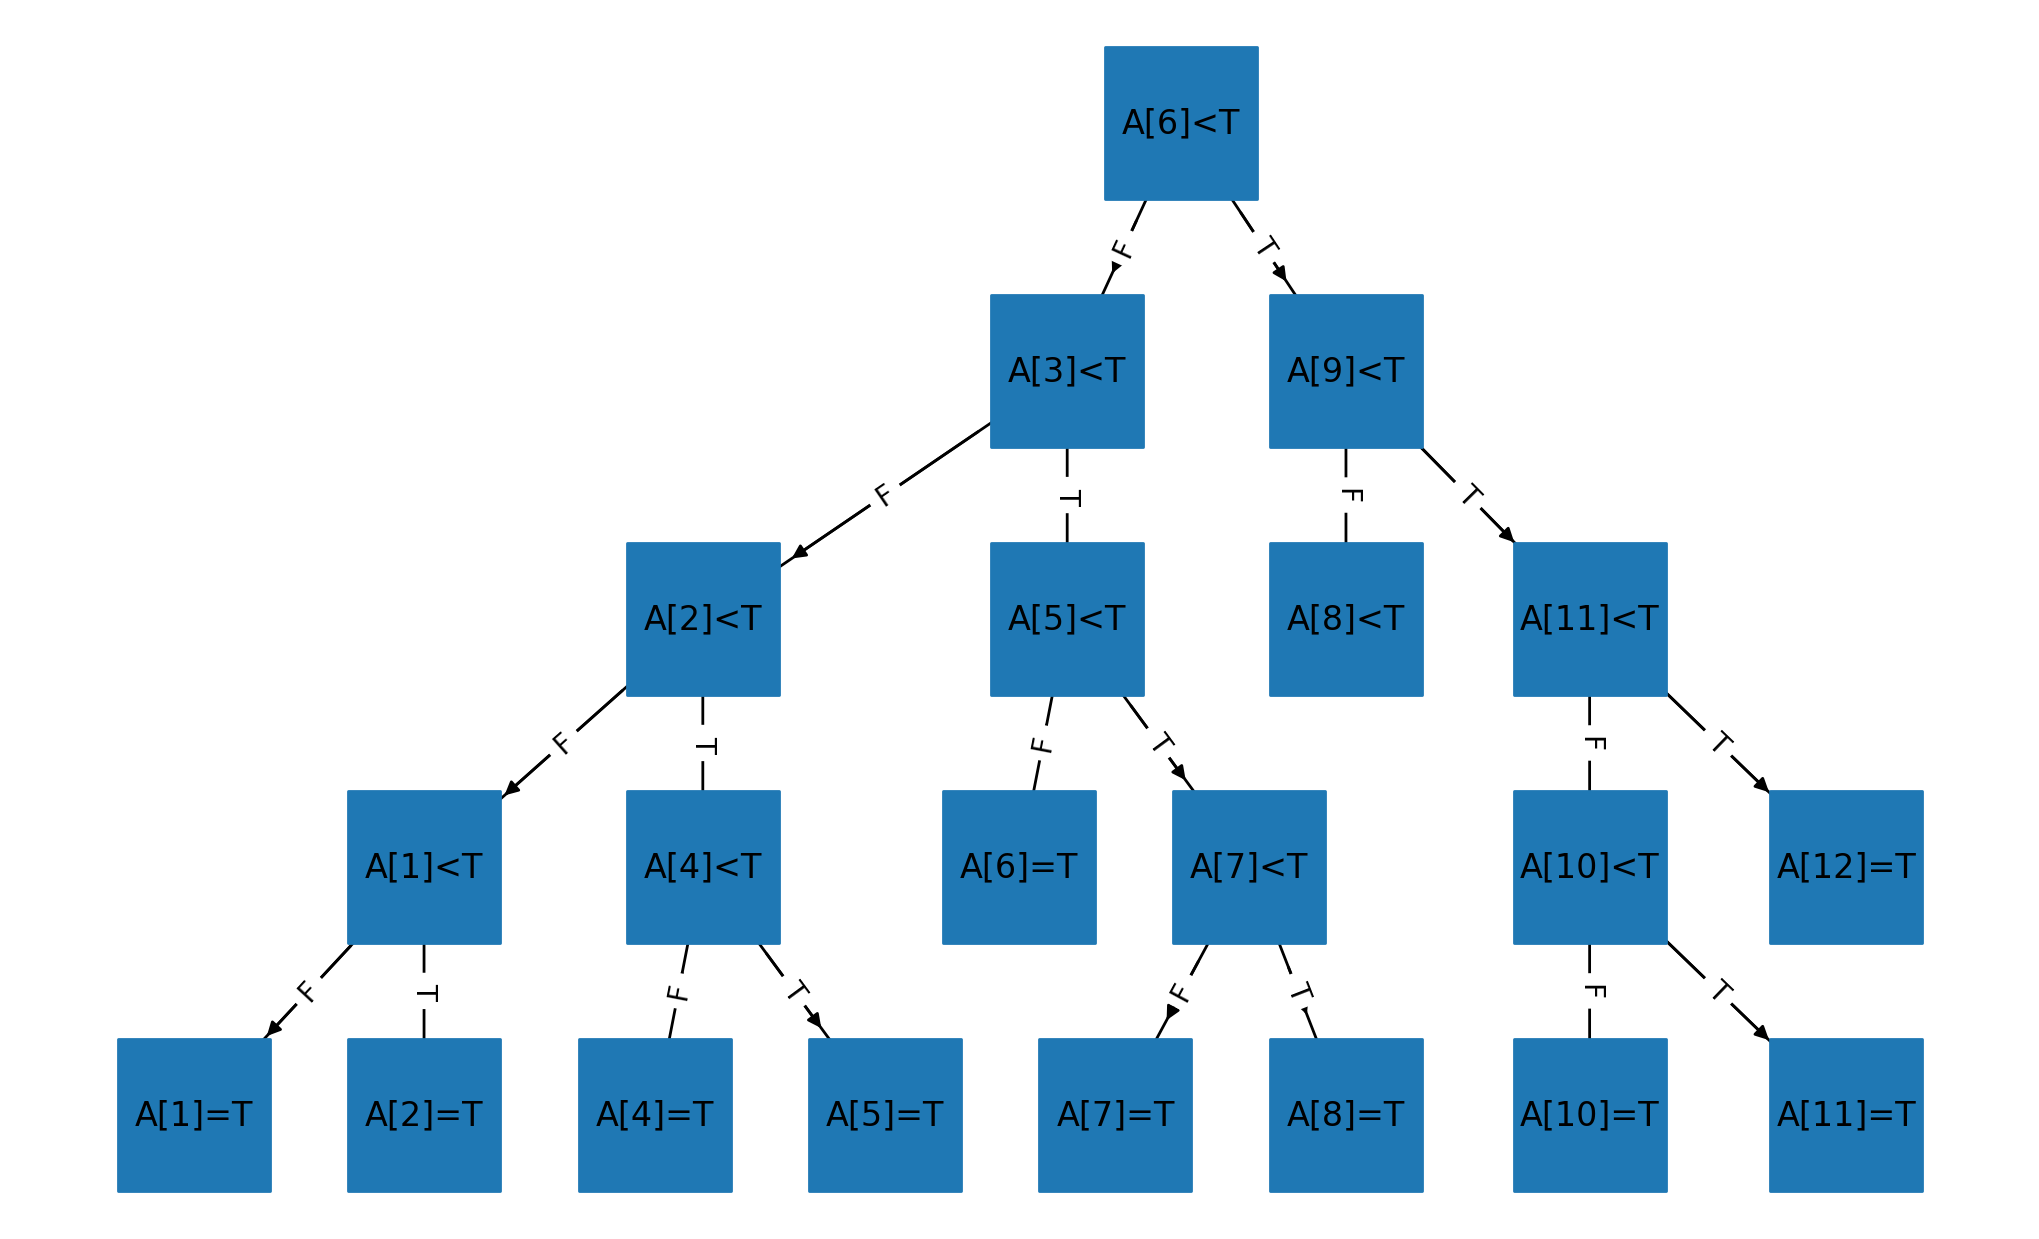
\includegraphics[width = 1\textwidth]{v2bintree.png}
        \caption{Binary Search V2 with $n=12$}
    \end{figure}
    This diagram is also a Binary Tree. But in it, from every internal vertex, there
    are exactly two edges downward in the diagram (never just one). This kind of
    Binary Tree is said to be a full Binary Tree. We will look into trees in detail in the next section.
    \begin{theorem}
        If \( T \) is a full binary tree with \( m \) internal vertices, then \( T \) has \( m + 1 \) leaves.
        \end{theorem}
        
        \begin{proof}
        We proceed by induction on the number of internal vertices, \( m \).
        
        \textbf{Base Case:} When \( m = 1 \), there is only one internal vertex, which is the root of the tree. By the definition of a full binary tree, the root must have two children, and since these children cannot be internal vertices (as there is only one internal vertex, the root itself), they must be leaves. Hence, the tree has \( 1 + 1 = 2 \) leaves, which satisfies our theorem.
        
        \textbf{Inductive Step:} Assume that the theorem holds for a full binary tree with \( m \) internal vertices, such that the tree has \( m + 1 \) leaves. Now consider a full binary tree with \( m + 1 \) internal vertices. By the definition of a full binary tree, adding an internal vertex means we are adding two children to an existing leaf (which is now converted into an internal vertex). This addition results in one less leaf (the converted internal vertex) and two more leaves (the new children). Therefore, the number of leaves increases by \( 2 - 1 = 1 \) compared to the number of leaves in the tree with \( m \) internal vertices.
        
        So, a tree with \( m + 1 \) internal vertices will have \( (m + 1) + 1 \) leaves. Hence, by the principle of mathematical induction, the theorem is true for all \( m \geq 1 \).
        \end{proof}
    \subsection{Exercises}
    \begin{exercise}
        Suppose \( T \) is not found by Binary Search. Where will \( T \) fit into the array? 
        Where should it be inserted?
    \begin{enumerate}
        \item Is the final \( q \)-value always one less than the final \( p \)-value?
        \item When is \( A[q] < T < A[p] \)?
        \item If \( p = 1 \) (that is, \( p \) was never changed), is \( T < A[1] \)?
        \item If \( q = n \) (that is, \( q \) was never changed), is \( A[n] < T \)?
    \end{enumerate}
    \end{exercise}
    
    \textbf{Solution}:
    \begin{enumerate}
        \item The final value of \( q \) is not necessarily always one less than the final \( p \) value. It depends on the search process and the position where \( T \) would fit if it were in the array.
        \item The condition \( A[q] < T < A[p] \) holds when \( T \) would be inserted between \( A[q] \) and \( A[p] \) in a sorted array to maintain the sorted order.
        \item If \( p = 1 \), it means \( T < A[1] \), and \( T \) should be inserted at the beginning of the array.
        \item If \( q = n \), it means \( A[n] < T \), and \( T \) should be inserted at the end of the array.
    \end{enumerate}


    \begin{exercise}
        Consider the best performance of binary search in $\Theta$ notation and worst performance in big $O$ notation. Is it possible to get the average performance in $\Theta$ notation? If yes, state the precise time complexity; if not, explain why.
    \end{exercise}
    \textbf{Solution:}

    \begin{itemize}
        \item Best time complexity: The best case scenario occurs when the target value is at the midpoint of the array, which happens with a constant time complexity, thus $\Omega(1)$. However, best case scenarios are generally not described using $\Theta$ notation as it implies a tight bound that is both the upper and lower limit, which is not applicable for the best case.
        \item Worst time complexity: Binary search has a worst-case time complexity of $O(\log n)$ when the target value is not within the initial bounds of the midpoint checks, thus requiring the maximum number of iterations to converge on the target.
        \item Average time complexity: The average time complexity of binary search is generally represented as $O(\log n)$. This is due to the fact that, on average, the number of steps required to find an element in a sorted array is logarithmic relative to the array size. Precise average case analysis of binary search is complex as it depends on the probability distribution of the target element's position. It is generally not represented in $\Theta$ notation because the lower and upper bounds for the average case cannot be tightly bounded as they can be for the best and worst cases.
    \end{itemize}
    
    \begin{exercise}
        Prove by MI that $\displaystyle \forall \ k\in \mathbb{N} ,\ $if Binary Search is applied to an array of length$\displaystyle \ n$ and has not terminated after $\displaystyle k$ (unsuccessful) probes, then the length of the current sublist must be less or equal to $\displaystyle \frac{n}{2^{k}}$
    \end{exercise}
    \begin{proof}
        We use $\displaystyle L(w)$ to denote the length of the current sublist after $\displaystyle w$ probes.
        
        \textbf{Base Case:}
        When $\displaystyle k=0$, the sorting is not yet started, so $\displaystyle L( 0) =n$, and we have $\displaystyle L( 0) =\frac{n}{2^{0}} =n$.
        
        \textbf{Inductive hypothesis:}
        Now assume that when $\displaystyle k=w$, it holds that:
        \begin{equation*}
        L( w) \leq \frac{n}{2^{w}}
        \end{equation*}
        
        \textbf{Inductive Step:}
        Thus, we need to prove that for $\displaystyle k=w+1$, $\displaystyle L( w+1) \leq 
        \frac{n}{2^{w+1}}$.
        We have proven earlier in theorem \ref{4.2.1} that after $\displaystyle w$ loops, $\displaystyle 
        \lfloor n/2^{w} \rfloor \leq L( w) \leq \lceil n/2^{w} \rceil $, and the length of the 
        sublist to be probed after $\displaystyle k+1$ unsuccessful probes is $\displaystyle 
        \frac{n}{2^{w+1}}$. While \ $\displaystyle \frac{n}{2^{w+1}} \leq \lceil n/2^{w+1} \rceil $. 
        Refer to the definition of $\displaystyle w( k)$ in the statement of problem, $\displaystyle 
        w\in \mathbb{N}$, so $\displaystyle \frac{n}{2^{w+1}} =\lceil n/2^{w+1} \rceil \ $. Hence, $\displaystyle L( w+1) \ \leq \frac{n}{2^{w+1}} \ $, this completes the proof.
    \end{proof}
    


